% This is "sig-alternate.tex" V2.0 May 2012
% This file should be compiled with V2.5 of "sig-alternate.cls" May 2012
%
% This example file demonstrates the use of the 'sig-alternate.cls'
% V2.5 LaTeX2e document class file. It is for those submitting
% articles to ACM Conference Proceedings WHO DO NOT WISH TO
% STRICTLY ADHERE TO THE SIGS (PUBS-BOARD-ENDORSED) STYLE.
% The 'sig-alternate.cls' file will produce a similar-looking,
% albeit, 'tighter' paper resulting in, invariably, fewer pages.
%
% ----------------------------------------------------------------------------------------------------------------
% This .tex file (and associated .cls V2.5) produces:
%       1) The Permission Statement
%       2) The Conference (location) Info information
%       3) The Copyright Line with ACM data
%       4) NO page numbers
%
% as against the acm_proc_article-sp.cls file which
% DOES NOT produce 1) thru' 3) above.
%
% Using 'sig-alternate.cls' you have control, however, from within
% the source .tex file, over both the CopyrightYear
% (defaulted to 200X) and the ACM Copyright Data
% (defaulted to X-XXXXX-XX-X/XX/XX).
% e.g.
% \CopyrightYear{2007} will cause 2007 to appear in the copyright line.
% \crdata{0-12345-67-8/90/12} will cause 0-12345-67-8/90/12 to appear in the copyright line.
%
% ---------------------------------------------------------------------------------------------------------------
% This .tex source is an example which *does* use
% the .bib file (from which the .bbl file % is produced).
% REMEMBER HOWEVER: After having produced the .bbl file,
% and prior to final submission, you *NEED* to 'insert'
% your .bbl file into your source .tex file so as to provide
% ONE 'self-contained' source file.
%
% ================= IF YOU HAVE QUESTIONS =======================
% Questions regarding the SIGS styles, SIGS policies and
% procedures, Conferences etc. should be sent to
% Adrienne Griscti (griscti@acm.org)
%
% Technical questions _only_ to
% Gerald Murray (murray@hq.acm.org)
% ===============================================================
%
% For tracking purposes - this is V2.0 - May 2012

\documentclass{sig-alternate}

\usepackage[noend]{algpseudocode}
\usepackage{caption}
\DeclareCaptionType{algorithm}

\begin{document}
%
% --- Author Metadata here ---
%\conferenceinfo{WOODSTOCK}{'97 El Paso, Texas USA}
\CopyrightYear{2013} % Allows default copyright year (20XX) to be over-ridden - IF NEED BE.
\crdata{}
%\crdata{0-12345-67-8/90/01}  % Allows default copyright data (0-89791-88-6/97/05) to be over-ridden - IF NEED BE.
% --- End of Author Metadata ---

\title{Large-scale Image Labeling via Mapreduce Topic Modeling}
\subtitle{[Spring 2012 CMSC828G Final Project Report]
\titlenote{Data-Intensive Computing with MapReduce instructed by Prof. Jimmy Lin}}
%
% You need the command \numberofauthors to handle the 'placement
% and alignment' of the authors beneath the title.
%
% For aesthetic reasons, we recommend 'three authors at a time'
% i.e. three 'name/affiliation blocks' be placed beneath the title.
%
% NOTE: You are NOT restricted in how many 'rows' of
% "name/affiliations" may appear. We just ask that you restrict
% the number of 'columns' to three.
%
% Because of the available 'opening page real-estate'
% we ask you to refrain from putting more than six authors
% (two rows with three columns) beneath the article title.
% More than six makes the first-page appear very cluttered indeed.
%
% Use the \alignauthor commands to handle the names
% and affiliations for an 'aesthetic maximum' of six authors.
% Add names, affiliations, addresses for
% the seventh etc. author(s) as the argument for the
% \additionalauthors command.
% These 'additional authors' will be output/set for you
% without further effort on your part as the last section in
% the body of your article BEFORE References or any Appendices.

\numberofauthors{3} %  in this sample file, there are a *total*
% of EIGHT authors. SIX appear on the 'first-page' (for formatting
% reasons) and the remaining two appear in the \additionalauthors section.
%
\author{
% You can go ahead and credit any number of authors here,
% e.g. one 'row of three' or two rows (consisting of one row of three
% and a second row of one, two or three).
%
% The command \alignauthor (no curly braces needed) should
% precede each author name, affiliation/snail-mail address and
% e-mail address. Additionally, tag each line of
% affiliation/address with \affaddr, and tag the
% e-mail address with \email.
%
% 1st. author
\alignauthor
Khoa Doan\titlenote{Dr.~Trovato insisted his name be first.}\\
       \affaddr{University of Maryland}\\
       \affaddr{Department of Computer Science}\\
       \affaddr{College Park, MD}\\
       \email{trovato@corporation.com}
%% 2nd. author
\alignauthor
Rahmatri Mardiko\titlenote{The secretary disavows
any knowledge of this author's actions.}\\
       \affaddr{University of Maryland}\\
       \affaddr{College Park, MD 20742}\\
       \email{mardiko@cs.umd.edu}
%% 3rd. author
\alignauthor 
Ang Li\titlenote{This author is the
one who did all the really hard work.}\\
       \affaddr{University of Maryland}\\
       \affaddr{Department of Computer Science}\\
       \affaddr{College Park, MD}\\
       \email{angli@cs.umd.edu}
%\and  % use '\and' if you need 'another row' of author names
%% 4th. author
%\alignauthor Lawrence P. Leipuner\\
%       \affaddr{Brookhaven Laboratories}\\
%       \affaddr{Brookhaven National Lab}\\
%       \affaddr{P.O. Box 5000}\\
%       \email{lleipuner@researchlabs.org}
%% 5th. author
%\alignauthor Sean Fogarty\\
%       \affaddr{NASA Ames Research Center}\\
%       \affaddr{Moffett Field}\\
%       \affaddr{California 94035}\\
%       \email{fogartys@amesres.org}
%% 6th. author
%\alignauthor Charles Palmer\\
%       \affaddr{Palmer Research Laboratories}\\
%       \affaddr{8600 Datapoint Drive}\\
%       \affaddr{San Antonio, Texas 78229}\\
%       \email{cpalmer@prl.com}
}
% There's nothing stopping you putting the seventh, eighth, etc.
% author on the opening page (as the 'third row') but we ask,
% for aesthetic reasons that you place these 'additional authors'
% in the \additional authors block, viz.
%\additionalauthors{Additional authors: John Smith (The Th{\o}rv{\"a}ld Group,
%email: {\texttt{jsmith@affiliation.org}}) and Julius P.~Kumquat
%(The Kumquat Consortium, email: {\texttt{jpkumquat@consortium.net}}).}
%\date{30 July 1999}
% Just remember to make sure that the TOTAL number of authors
% is the number that will appear on the first page PLUS the
% number that will appear in the \additionalauthors section.

\maketitle
\begin{abstract}
Large scale computer vision is recently being popular due to the emerging of large scale imagery data and in need of more generally trained visual models.
Recent advances in feature extraction provide a feasible and succinct way to represent image regions. However, most of these features are computationally heavy to extract. Since there is no explicit method to essentially speed up feature extraction, parallelization becomes the most comfortable strategy for this task.
Due to the inherent high dimensionality of visual data, extracted features can be very noisy and thus not representative for images. Feature quantization is introduced to group similar features into the same low level semantics. K-means clustering is one of the usual choices for quantization while it may suffer from either time or space problems in ordinary environment. Latent Dirichlet Allocation is one of the techniques to discover higher level topic semantics for the context, which was popular in natural language processing. In this project, we unearth the potential of adapting computer vision tasks such as low level feature extraction and higher level image understanding into the MapReduce framework for large scale image dataset. We adopt the MapReduce LDA (Mr.LDA) to find topics across the images and discuss its possible extensions with respect to the image domain.


\end{abstract}

% A category with the (minimum) three required fields
%\category{H.4}{Information Systems Applications}{Miscellaneous}
%A category including the fourth, optional field follows...
%\category{D.2.8}{Software Engineering}{Metrics}[complexity measures, performance measures]

%\terms{Theory}

\keywords{Topic modeling, image labeling, parallelization, MapReduce framework}

\section{Introduction}
Large scale visual data analysis and machine learning have been recently received much attention during the past few years. Traditional computer vision research focuses on small datasets of images or videos which makes the generalization of these methods difficult. In the current world of big data, a lot of imagery data have been present in the Internet. How to make use of the large scale of data to explore a better visual model has been one of the central problems in the current community. However, one natural problem arised from this task is heavy computational load. Computer vision tasks are usually involved with feature engineering which requires a lot of time and space for experiments. Fortunately, the MapReduce framework provides a reliable approach to large scale data processing.

In this work, we explore the potentials of using MapReduce framework for a standard computer vision task i.e. image labeling. The objective of the image labeling task is to find underlying semantics for each of the image pixels and to find groups of pixels that belong to the same object or semantic. Image labeling has been investigated for decades, although the scale of the dataset is limited due to computational issues. However, the demand of large scale image labeling turns out to be more and more clear in the recent years. One of the reasons is that people are being aware of using computer techniques to assist human annotation for specific imagery data such as remote sensing data. Millions of satellite images are generated for every day and the task of understanding these data is never feasible for human to do exhaustively. The automatic way will benefit the community tremendously in different areas such as surveillance, city planning, national defense, etc.

The rest of this paper is organized as follows.
Section \ref{sec:overview} briefly introduces the system structure of this project.
MapReduce framework for visual feature extraction is discussed in section \ref{sec:feature}.
Details of Mr.LDA is introduced in section \ref{sec:mrlda}. In section \ref{sec:impl}, a few implementation details are
discussed. Section \ref{sec:exp} shows the evaluation methods and experimental results for this project. Discussion on
possible extensions from LDA to Spatial LDA is presented in section \ref{sec:slda}. Finally, the paper concludes in section \ref{sec:con}.

\section{System Overview}\label{sec:overview}

\section{Feature Extraction}\label{sec:feature}
Feature extraction often dominates the most computational resources in computer vision tasks. In this section, we introduce a MapReduce based framework to extract visual features efficiently which distributes the computation loads for raw feature extraction and scales up the construction of feature codebook via MapReduce K-means clustering.
\subsection{Scale Invariant Feature Transform (SIFT)}
In this work, the Scale Invariant Feature Transform (SIFT) \cite{sift} is adopted to describe local regions across the images. Generally, a SIFT descriptor represent a region bounded by a rectangular box centered at $(x_c,y_c)$. The bounding box is uniformly divided into $K\times K$ parts. The gradients are computed in these sub-regions and the gradient magnitudes in $N_b$ (the number of bins) discretized orientations  are computed. A histogram is then constructed to represent the distribution of the gradient magnitudes. Therefore, for each region, the SIFT descriptor is a $K^2N_b$ dimensional histogram vector. Figure \ref{fig:sift} illustrates the SIFT feature computation.

\begin{figure}[!htb]
\centering
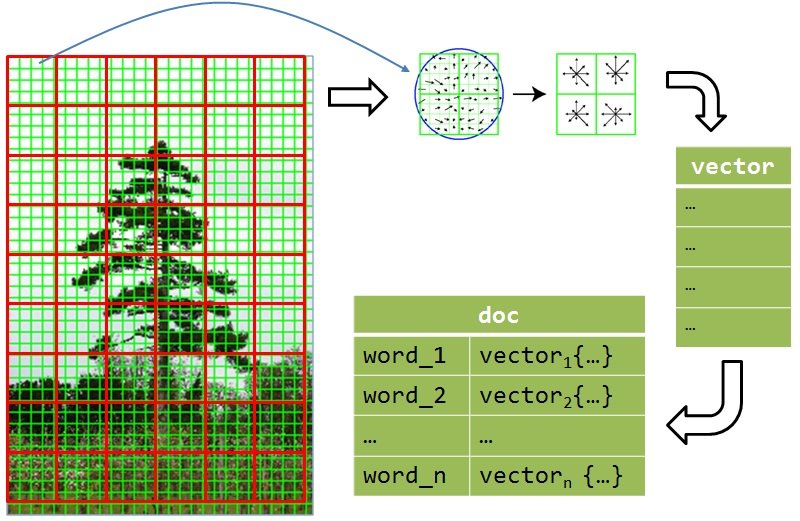
\includegraphics[width=0.48\textwidth]{fig/sift-extract}
\caption{Illustration of SIFT feature extraction}\label{fig:sift}
\end{figure}

One of the advantages of SIFT descriptors is its invariance to image rotation and translation, which makes this feature very popular among the computer vision community. We base our project on the MPI-CBG JavaSIFT library\cite{mpicbg}.
\subsection{Dense Sampling SIFT Features}
In order to apply SIFT features to represent the whole image for the task of image labeling, each of the pixels ideally should be described. Due to the fact that a neighborhood of pixels usually have little difference and belong to the same semantics, we sample series of small rectangular regions with a parameter \textsc{stepsize} densely across each of the image and compute the SIFT description for each of the regions. The \textsc{stepsize} controls the number of pixels between two consecutive centers of bounding boxes. Thereafter, each image can be converted from visual data to a list of \textsc{(key,value)} pairs where the \textsc{key} is the index $(g_i,x_i,y_i)$ of the regions and the \textsc{value} is the SIFT feature vector $f_i$. $g_i$ is the id of the image that contains the $i$-th region and $(x_i,y_i)$ is the center location of the $i$-th region.

\subsection{Image Input Aggregation}
Given a large number of image files as input, there are several ways of loading them into a MapReduce job. One possible way is creating a text file containing a list of file names and let the mapper reads the files from HDFS and processes them while the reducer does nothing. An alternative way is similar to the first except the reading and processing is moved to the reducer while the mapper just passes the (key,value) pairs. Both are relatively simple and easy to implement. However, due to the small-files problem in Hadoop\cite{smallfiles}, neither the first and the second approach achieves the best performance in terms of processing speed. 

Since Hadoop framework works best with large files, we need to aggregate the images in the dataset into a few big files. This step allows us to speed-up the feature extraction (and other images processing tasks) given a large number of image files as input. We adopt the approach presented in\cite{combinefiles} which creates a MapReduce job that packs multiple files into a \texttt{SequenceFile}. This aggregation is performed as a preprocessing step for the other jobs that take images as input.

\subsection{MapReduce-based Feature Extraction}
A list of image paths is generated in order to locate the image files. Each of the paths is assigned a number as image ID. The MapReduce job takes the path list as input and output sequence files containing region indices as keys and SIFT feature descriptors as values.

\begin{algorithm}[!htb]
\caption{Mapreduce Feature Extraction}
\begin{algorithmic}
\rm
\Function{mapper}{LongWritable \texttt{key}, Text \texttt{value}}
\State (\texttt{id}, \texttt{path}) = \textsc{Split}(\texttt{value}, \texttt{'\char`\\t'});
\State \textbf{emit} (\texttt{id}, \texttt{path});
\EndFunction
\end{algorithmic}
\vskip 1em
\begin{algorithmic}
\rm
\Function{reducer}{IntWritable \texttt{key}, Text \texttt{value}}
\State \texttt{id} = \texttt{key};
\State \texttt{image} = \textsc{ReadImageFromHDFS}(\texttt{value});
\State \texttt{feature} = \textsc{ExtractDenseSIFT}(\texttt{image});
\State \textbf{emit} (\texttt{id}, \texttt{feature});
\EndFunction
\end{algorithmic}
\end{algorithm}
\subsection{Building Feature Codebook}
The raw features extracted from above generally have two problems in representing the images. On the one hand, the dimension of each feature vector is typically 128. For the similarity measure of each pair of small regions, at least 128 times of multiplications are necessary for Euclidean distances. This makes the further processing intractable even using parallelization framework. On the other hand, the feature vector is a histogram of oriented gradients which contains a lot of noises. Therefore, feature quantization is introduced to further processing the features and construct a "codebook" for the features. In the codebook, nearby feature vectors are grouped into the same index because they should belong to the same visual semantics.

K-means clustering is usually the choice for doing feature quantization. However, the clustering takes more features and thus needs much more memory spaces in order to exhaustively compute the distances between cluster centers to each of the points, as the scale of data becomes larger. The MapReduce framework generally resolve this time and space problem because not only the computation is distributed into different nodes but also the intermediate results of distances are stored almost uniformly among all of the nodes. In our project, we adopt Mahout K-means clustering \cite{mahout} for building the codebook in Hadoop environment.
\section{MapReduce LDA}\label{sec:mrlda}
\cite{mrlda}

\section{MapReduce Spatial LDA}
%\begin{equation}
%\begin{split}
%q(\phi,\pi,d,z &| \lambda,\gamma,\eta,\varphi) = \\
%&\prod\limits_{k=1}^{K}q(\phi_k|\lambda) \: \prod\limits_{m=1}^{M}q(\pi_m|\gamma) \: \prod\limits_{n=1}^{N}q(d_n | \eta) q(z_n | \varphi)
%\end{split}
%\end{equation}
%where $\phi_k \in R^V$ is distribution over word of topic $k$, $\pi_m \in R^K$ is distribution over topics of document $m$, $d_n \in R^M$ is indicator vector where if $d_{nm} = 1$ means word $n$ belongs to document $m$, and $z_n \in R^K$ is indicator vector where if $z_{nk} = 1$ means word $n$ is assigned to topic $k$.

\section{Implementation Remarks}\label{sec:impl}
In this section we present some implementation details that we did in the project.
\subsection{Images to Pixels Conversion}
In the evaluation phase of the project we need to compare the LDA output and the true labels. To enable pixel-by-pixel evaluation we extract each pixel in the ground truth images and store them as (key,value) pairs. The key, which contains the image id and the pixel position ($x$,$y$), is of type \texttt{TripleOfInts} whereas the value is of type \texttt{IntWritable} and it contains the pixel value. This images-to-pixels conversion can actually be performed as map-only MapReduce job. However, sometimes it is useful to group pixels that have the same semantic together. Here we can apply value-to-key conversion so the pixels that have the same labels are grouped together when they arrive at the reducer.

\begin{algorithm}[!htb]
\caption{MapReduce Convert Images to Pixels}
\begin{algorithmic}
\rm
\Function{mapper}{IntWritable \texttt{key}, BytesWritable \texttt{value}}
\State \texttt{image} = \textbf{read}(\texttt{value});
\State \texttt{width,height} = size(\texttt{image});
\For{$y = 1 \to \texttt{height}$}
\For{$x = 1 \to \texttt{width}$}
\State \texttt{pixel} = \textbf{getpixel}\texttt{(image,x,y)};
\State \textbf{emit} (\texttt{pixel}, \texttt{(key,x,y)});
\EndFor
\EndFor
\EndFunction
\end{algorithmic}
\vskip 1em
\begin{algorithmic}
\rm
\Function{reducer}{IntWritable \texttt{key}, Iterable<TripleOfInts> \texttt{values}}
\State \texttt{iter} = \textbf{iterator}(\texttt{values})
\While{\texttt{iter.hasNext()}}
\State \textbf{emit} (\texttt{iter.next()}, \texttt{key});
\EndWhile
\EndFunction
\end{algorithmic}
\end{algorithm}

\subsection{Pixels to Images Conversion}
Also for the evaluation purpose, we need to build images from a set of pixels. This task is the inverse of the previous task. The mapper takes ((image\_id,x,y),pixel) pairs and produce (image\_id,(x,y,pixel)) as intermediate key value pairs so the pixels that belong to the same image are grouped together in the reducer. In the reducer the pixels are used to build the image object and convert it to \texttt{BytesWritable}. Since the output is in the form of \texttt{SequenceFile}, we still need to read the output separately to get the individual image files.

\begin{algorithm}[!htb]
\caption{MapReduce Convert Pixels to Images}
\begin{algorithmic}
\rm
\Function{mapper}{TripleOfInts \texttt{key}, IntWritable \texttt{value}}
\State \texttt{image\_id,x,y} = getmembers(\texttt{key});
\State \textbf{emit} (\texttt{image\_id}, \texttt{(x,y,value)});
\EndFunction
\end{algorithmic}
\vskip 1em
\begin{algorithmic}
\rm
\Function{reducer}{IntWritable \texttt{key}, Iterable<TripleOfInts> \texttt{values}}
\State \texttt{image} = \textbf{new image}(\texttt{width,height});
\State \texttt{iter} = \textbf{iterator}(\texttt{values})
\While{\texttt{iter.hasNext()}}
\State \texttt{x,y,pixel} = \textbf{getmembers}(\texttt{value});
\State \textbf{setpixel}(\texttt{image,x,y,pixel});
\EndWhile

\State \texttt{imseq} = \textbf{getbytes}(\texttt{image});
\State \textbf{emit} (\texttt{key}, imseq);
\EndFunction
\end{algorithmic}
\end{algorithm}

\section{Experimental Evaluation}\label{sec:exp}
\subsection{Dataset}
\subsubsection{MSRC Image Labeling Dataset}
The MSRC image labeling dataset (version 1) \cite{msrc} contains 240 images and 9 object classes in total. 
Each of the images is pixel-wise labeled. Fig.(\ref{fig:msrc}) shows some sample images from MSRC dataset.
\begin{figure}[!htb]
\centering
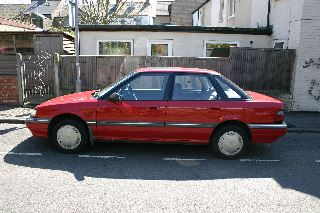
\includegraphics[width=0.11\textwidth]{fig/sample-msrc1}
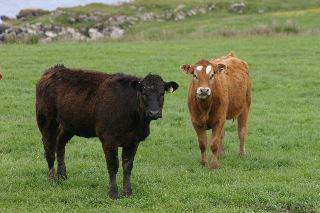
\includegraphics[width=0.11\textwidth]{fig/sample-msrc2}
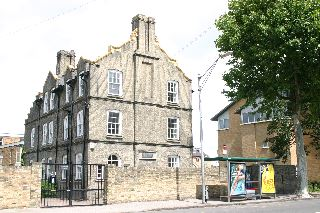
\includegraphics[width=0.11\textwidth]{fig/sample-msrc3}
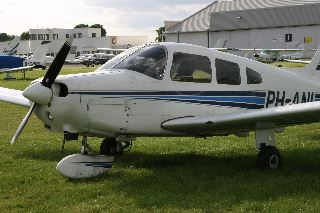
\includegraphics[width=0.11\textwidth]{fig/sample-msrc4}
\caption{Sample images from MSRC Image Labeling Dataset}\label{fig:msrc}
\end{figure}
\subsubsection{Eastern Coast Satellite Image Dataset}
We also collect satellite images using Google Maps APIs along the eastern coast in the United States. Each of the image is of 8-bit colormap PNG format and contains $402\times415$ pixels. Due to the capacity of our cluster, we pick 10,000 images amongst the dataset for the experiments. Fig.(\ref{fig:gmaps}) shows some sample images from Satellite image dataset.
\begin{figure}[!htb]
\centering
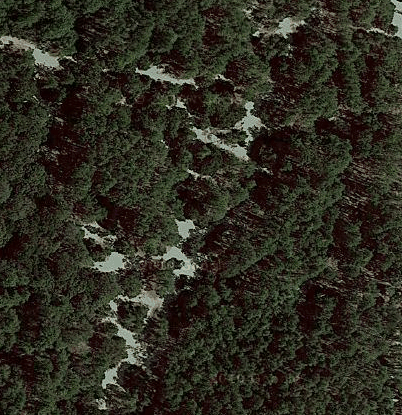
\includegraphics[width=0.11\textwidth]{fig/sample-gmaps1}
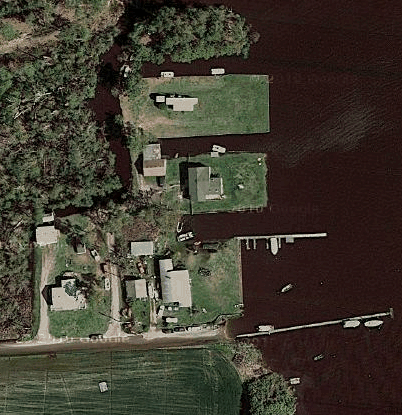
\includegraphics[width=0.11\textwidth]{fig/sample-gmaps2}
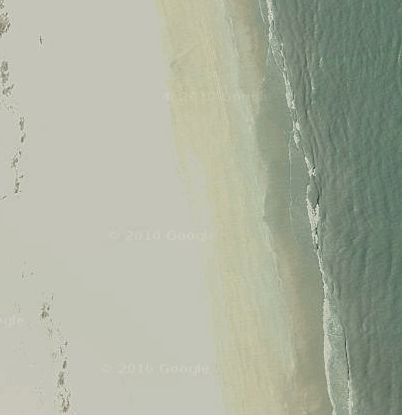
\includegraphics[width=0.11\textwidth]{fig/sample-gmaps3}
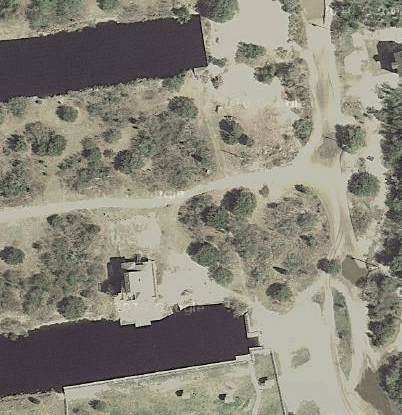
\includegraphics[width=0.11\textwidth]{fig/sample-gmaps4}
\caption{Sample images from Eastern Coast Satellite Image Dataset}\label{fig:gmaps}
\end{figure}

\subsection{Qualitative Evaluation}
Images with labels in different colors are recovered from the output of LDA to show qualitatively which parts belong to the same semantics. Figure \ref{fig:qual} presents three sample images and the output labels with 9 and 14 topics. The ground truth consists of 14 distinct semantics. However, the performance of LDA is significantly higher with 9 topics than 14 topics.
\begin{figure}[!htb]
\centering
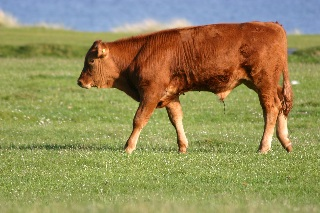
\includegraphics[width=0.11\textwidth]{fig/125-origin}
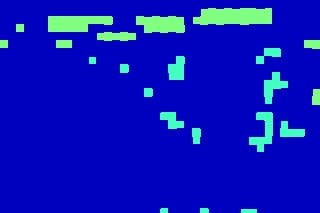
\includegraphics[width=0.11\textwidth]{fig/125-lda-topic14}
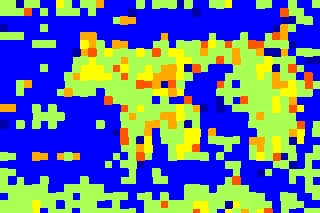
\includegraphics[width=0.11\textwidth]{fig/125-lda-topic9}
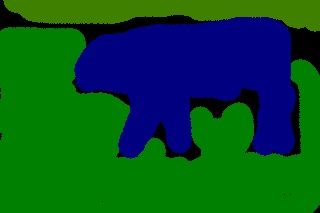
\includegraphics[width=0.11\textwidth]{fig/125-GT}\\
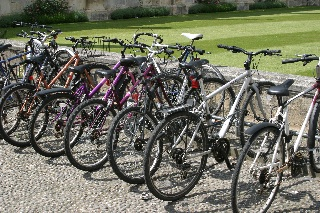
\includegraphics[width=0.11\textwidth]{fig/216-origin}
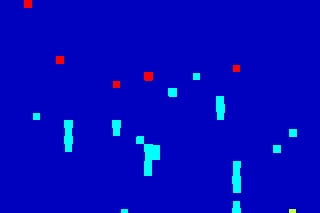
\includegraphics[width=0.11\textwidth]{fig/216-lda-topic14}
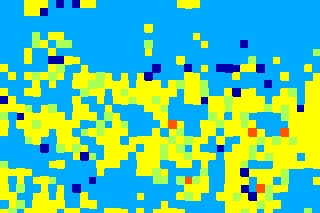
\includegraphics[width=0.11\textwidth]{fig/216-lda-topic9}
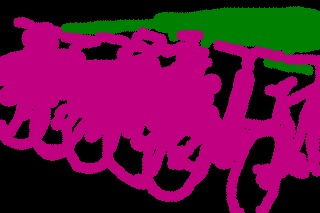
\includegraphics[width=0.11\textwidth]{fig/216-GT}\\
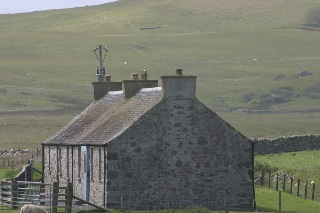
\includegraphics[width=0.11\textwidth]{fig/65-origin}
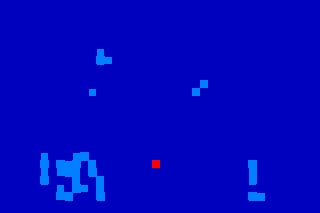
\includegraphics[width=0.11\textwidth]{fig/65-lda-topic14}
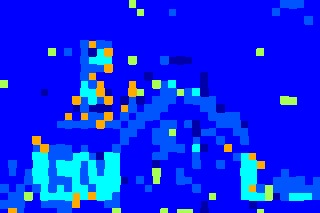
\includegraphics[width=0.11\textwidth]{fig/65-lda-topic9}
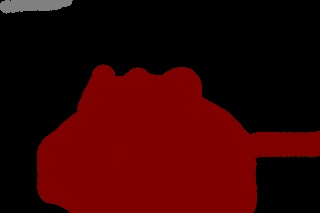
\includegraphics[width=0.11\textwidth]{fig/65-GT}
\caption{Sample LDA output from MSRC dataset. The second and the third column show the output of labeling with LDA using 14 and 9 topics. The last column show the ground truth images.}\label{fig:qual}
\end{figure}

\subsection{Quantitative Evaluation}
Traditional computer vision dataset has ground-truth for evaluation. For the MSRC image labeling data, each image is corresponded to a groundtruth image in which the whole image is divided into several components. Each component is annotated using a unique RGB color. In our output, each pixel is assigned to a type of semantics. Since our approach is completely unsupervised, the truth meaning of each semantic is not understandable. One possible way to evaluate the performance is to enumerate every possible correspondence between the two set of semantics. Apparently this strategy only works when the number of topics is small enough. It becomes difficult to construct a one-one correspondence between our labels and the groundtruth labels. In fact, how to accurately evaluate the performance of image segmentation tasks is still an open problem.

In this project, we propose to evaluate the results for each of the topics separately. For each semantic in the ground truth, a binary image can be constructed, regions with value 1 are those containing such semantic and otherwise not. For the output of the resulted topics, the topic that has the most number of occurrences in the semantic regions are chosen as a correspondence. The precision and recall are then computed according to that topic.
\begin{align}
\text{precision}&=\frac{\text{\#TruePositive}}{\text{\#TruePositive+\#FalsePositive}}\\
\text{recall}&=\frac{\text{\#TruePositive}}{\text{\#TruePositive+\#FalseNegative}}
\end{align}
\section{Discussion: Spatial Latent Dirichlet Allocation}\label{sec:slda}

\section{Conclusion}\label{sec:con}

%\begin{table}
%\centering
%\caption{Frequency of Special Characters}
%\begin{tabular}{|c|c|l|} \hline
%Non-English or Math&Frequency&Comments\\ \hline
%\O & 1 in 1,000& For Swedish names\\ \hline
%$\pi$ & 1 in 5& Common in math\\ \hline
%\$ & 4 in 5 & Used in business\\ \hline
%$\Psi^2_1$ & 1 in 40,000& Unexplained usage\\
%\hline\end{tabular}
%\end{table}



%ACKNOWLEDGMENTS are optional
\section{Acknowledgments}
The authors would like to thank Prof. Jordan Boyd-Graber and Prof. Jimmy Lin for their consistent help in this project.

%
% The following two commands are all you need in the
% initial runs of your .tex file to
% produce the bibliography for the citations in your paper.
\bibliographystyle{abbrv}
\bibliography{sigproc}  % sigproc.bib is the name of the Bibliography in this case
% You must have a proper ".bib" file
%  and remember to run:
% latex bibtex latex latex
% to resolve all references
%
% ACM needs 'a single self-contained file'!
%
%APPENDICES are optional
%\balancecolumns
\appendix
%Appendix A
%\section{Headings in Appendices}
\end{document}
